\chapter{Potential Development and Pareto Optimality}

In the previous chapter, an overview of the different computational tools associated to atomistic simulation were presented to give some idea of interconnectivity and breath of atomistic simulations.  Within this chapter, we outline the Pareto approach to potential optimization within the context of more typical current appraoches to potential development.

This chapter frames potential development using a broad mathematical treatment.  The purpose is to frame some of the problems in potential development in the proper context as to understand the limitations of typical approaches in potential development.  Parameterization is often approaches to the minimization of a scalar objective functions consisting of the weighted sum of square differences with respect to the prediction of a set of material properties.  When the gradient is continuously differentiable with respect to its parameters and the objective function is convex, the gradient approach is relatively efficient, even in high dimension.  For interatomic potentials, these conditions are most likely not guaranteed for even fairly simple formulae to represent the interactions between atoms.  This necessitates the implementation of global optimization approaches to the minimization, drastically increasing the computational time for even a single selection of weights.

Moreover, gradient approaches to optimization are not amenable to parallelization.  The approach starts at an initial condition and improves the estimate in an iterative manner.  As a result, the parallelization of the computational effort is limited by the dimensionality of the parameter space (length of the computation of the gradient) and limited to the number of simulations required to compute each material property.  This limits the processor utilization to $(M \times N)$, where $M$ is the number of simulations required to calculate the cost function, and $N$ is the length of parameter space.

A larger problem is the weighted least squares approach makes parameterization dependent upon the selection of weights, which determines the optimal parameterization.   The weights expresses the preferences of the potential developer which must be expressed \emph{a priori}.  Some methods have been developed to pre-determine weights which incorporate the magnitude and acceptable errors of the target properties and a rough sense of properties.  In practice, a initial choice of weights is made based on the experience of the potential developer and the weights varied with respect the magnitude of the target until an acceptable parameterization is achieved.

To address the issues of this approach, a novel approach to parameter optimization is taken which incorporates two pieces.  First, since gradient based scalar optimization is problematic, we recast the problem as a multi-objective optimization problem (MOO), where each of the subobjectives in the cost function are treated indpendently.  The concept of a single optimal parameterization is clearly an inappropriate representation since the objective functions are conflicting.  As a result, the solution to a MOO must be an ensemble of parameterizations; each optimal in it's own way.  This set of optimal potentials is defined as Pareto optimal.  Second, while the Pareto optimal can be estimated by varying the weights in the cost function in a systematic way, such an approach is likely inefficient due to the problems with gradient based optimization.  Instead, a sampling based approach is proposed.

This chapter consists of three sections.  In the first section, we introduce the idea of a potential energy surface and how interatomic potentials can be thought of as computational inexpensive surrogate models, and we introduce the terminology of potential development as well as some broad concepts of potential optimization.

Next, we build up the notation and terminology of general optimization from a broad mathematical standpoint, first covering the more familiar single-objective optimization.  In particular, we discuss the the current techniques to potential optimization which are applied to potential optimzation as well as some of the mathematical problems and issues of this approach.

Finally, the problem of a parameterization is defined within the context of a MOO problem, with the solution of MOO being the set of parameters which produce the Pareto optimal set.  When the Pareto surface is convex and continuously differentiable, gradient based approaches can estimate the Pareto surface.  When these conditions do not exist, gradient based approaches produces erroneous results.  As a preview to the evolutionary method presended in chapter \ref{chap5}, we demonstrate how a random sampling based approach to optimization is likely a better approach to estimating a Pareto optimal surface when the potential developer has a high degree of uncertainty to the selection of a region of potential parameterizations or weighting vectors.  This is demonstrated through some sample calculations on the continuous, convex MOO  problem of Schaffer\cite{schaffer1984_pareto} and the discontinuous, nonconvex MOO problem of Kurasawe\cite{kursawe1001_pareto} and the  detail of these functions is contained in Appendex \ref{ap:pareto optimization_test}

\section{Potential Energy Surfaces}

To study the evolution of a system, such as kinetic properties and chemical reactions, it is necessary to calculate the energy for every atomic arrangement of interest.  The potential energy surface is the energy of a collection of atoms as a function of the positions of its nuclei, $\{\bm{R}\}$.
A PES represents a mapping of the positions of the atoms of a material system to an energies, $V:\{\bm{R}\}\rightarrow E$, with $E\in\mathbb{R}$.
Given an atomic arrangement $\bm{R}$, the evaluated potential surface $V(\bm{R})$ gives the height of the energy landscape for any atomic configuration, providing an approximation of the potential energy surface, so that the concept of a potential energy surface arises.
This creates an energy landscape which allows materials systems to viewed from a topological perspective, which allows the PES to describe the evolution of a system as it moves from one atomic configuration to another atomic configuration.

To describe empirical potentials, we first start with a a mathematical description of configuration space both from a crystallographic perspective, but how this crystallgraphic perspective can be translated into other representation common with empirical potentials.

\section{Configuration Space}
In solid materials, atoms are typically represented as infinite crystalline solids, with th atomic positions placed within a representative unit volume.
This representative unit is referred to as a unit cell, which defines that boundaries, the volume, the lattice positions of each atom.

\begin{figure}[h]
	\centering
  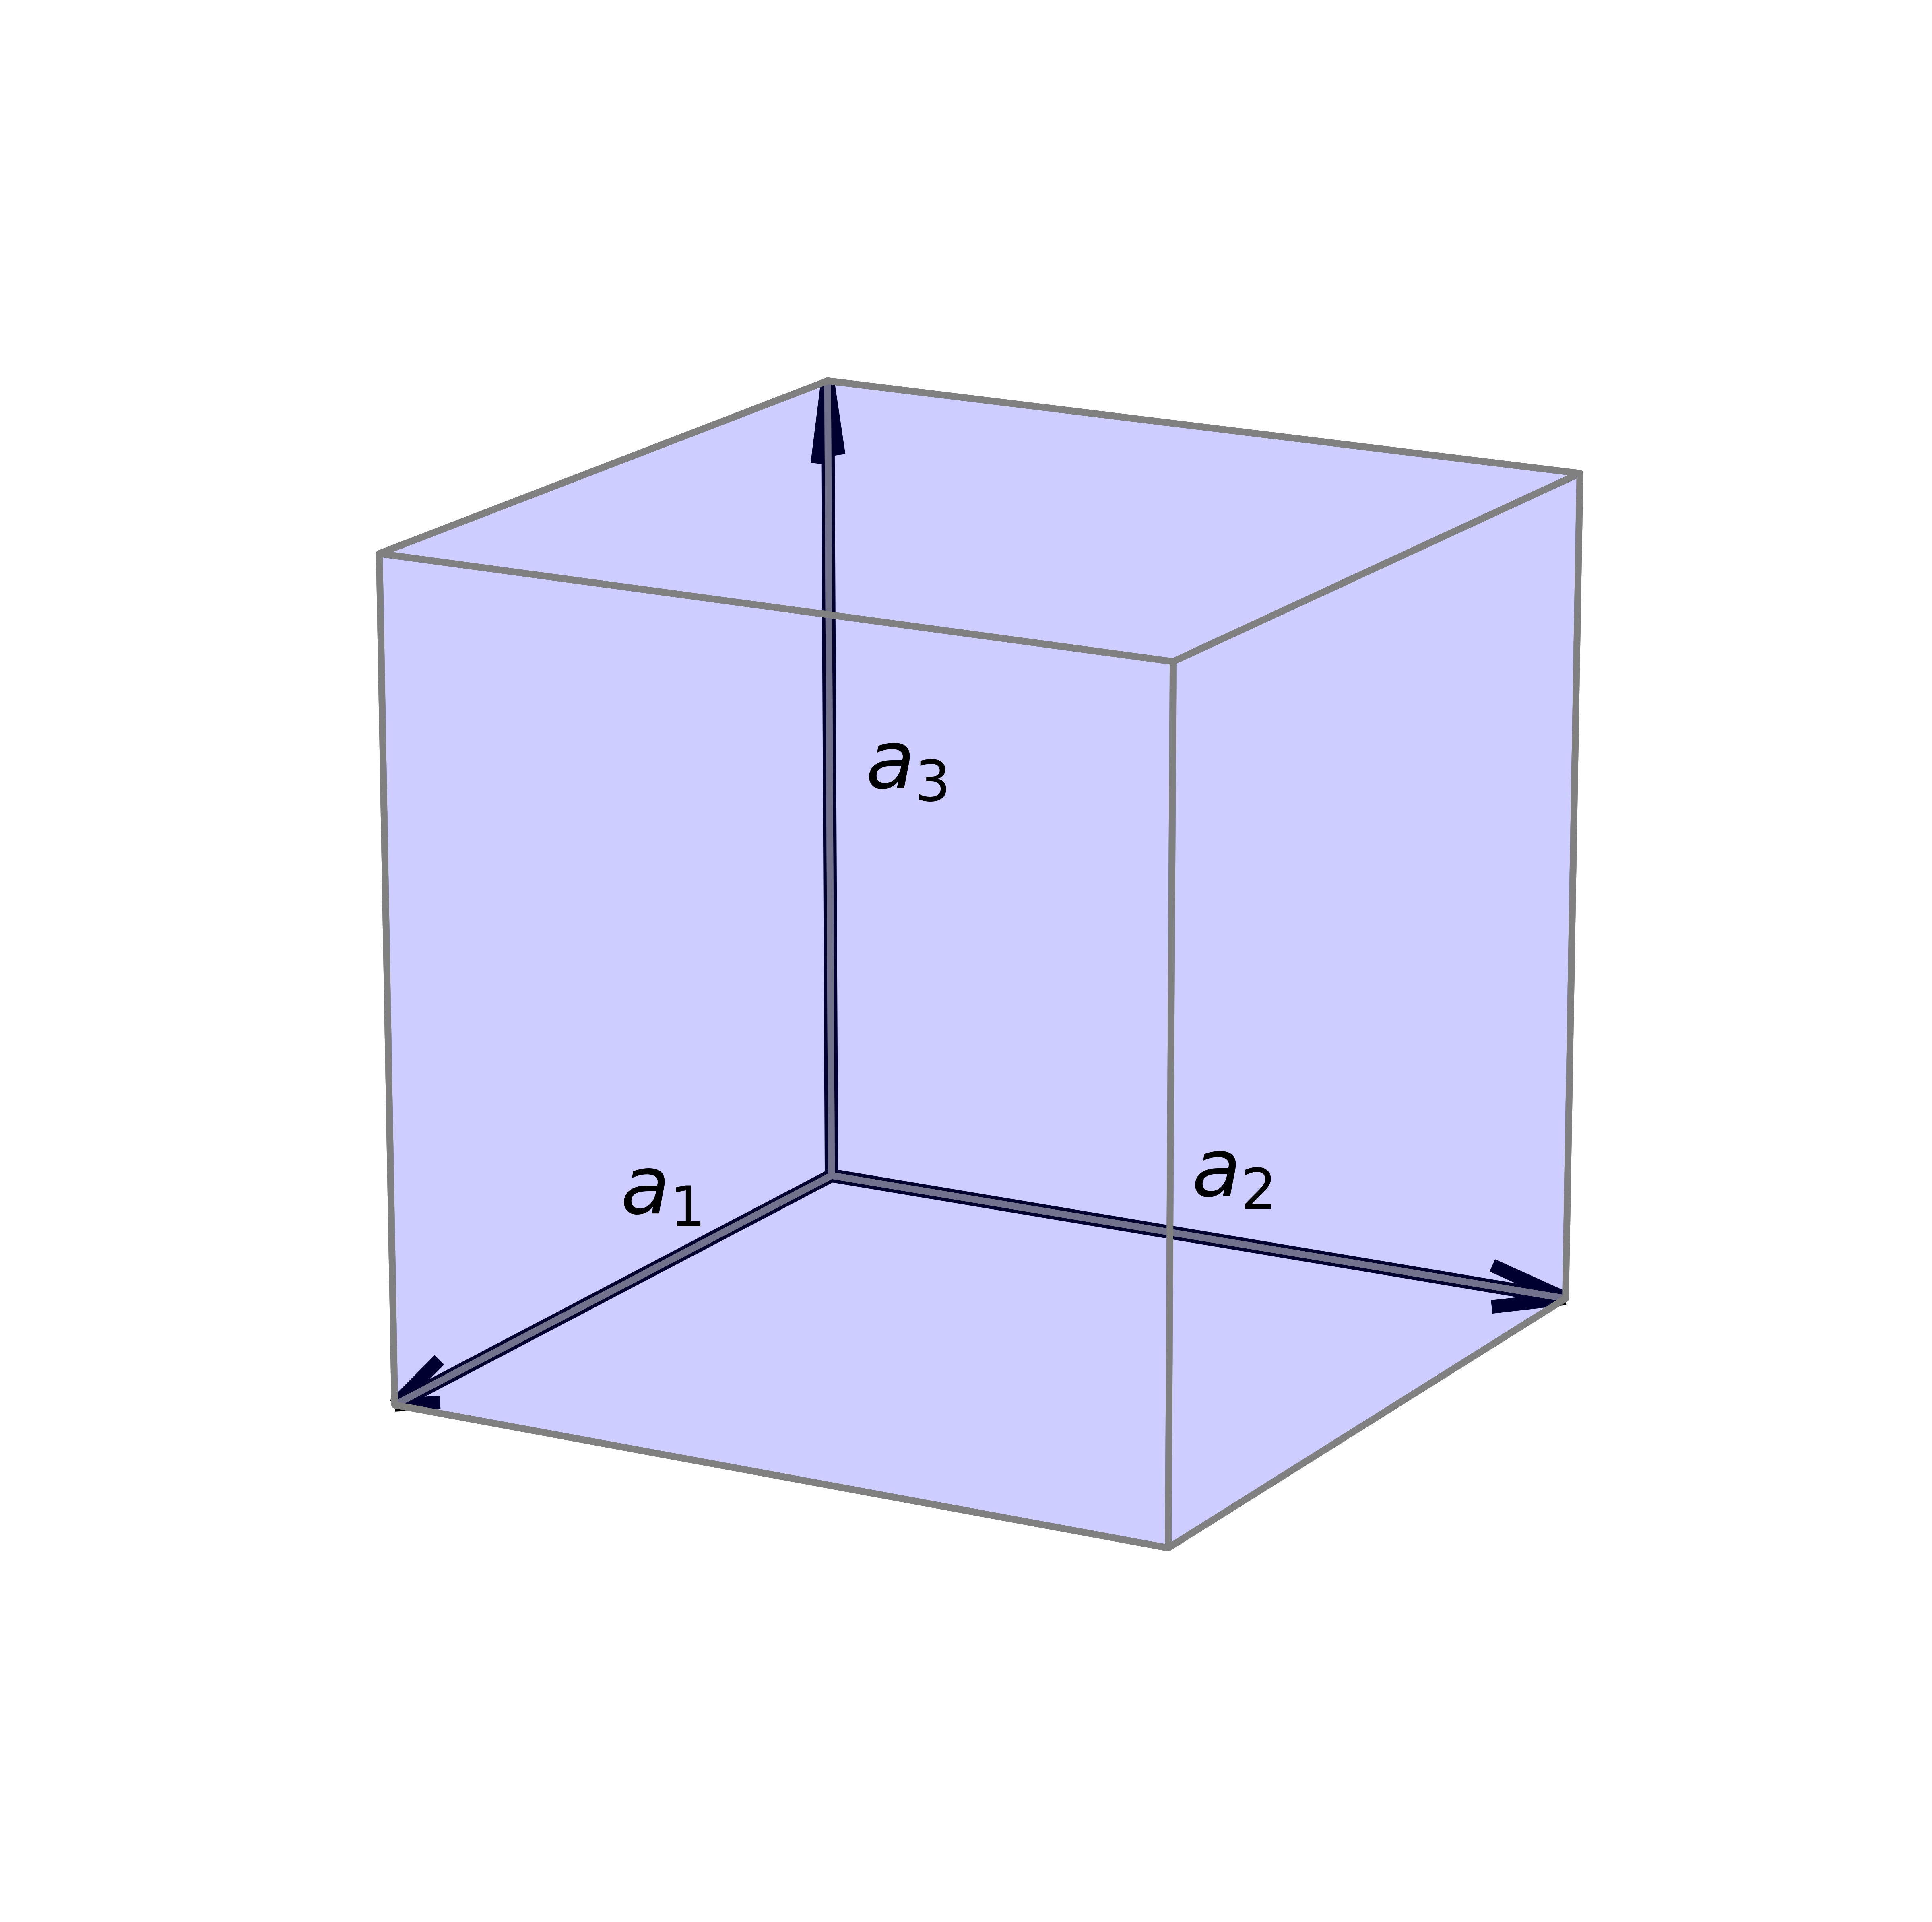
\includegraphics{chapter3/unit_cell}
  \caption{Depiction of the lattice vectors which bound the the unit cell depicted in blew.}
  \label{fig:unit_cell}
\end{figure}

The boundaries of the unit cell are defined are defined by three lattice vectors, defined in three dimensional Euclidean space, $\mathbb{R}^3$.
The three lattice vectors, $\bm{a}_1$, $\bm{a}_2$, and $\bm{a}_3$, with $\bm{a_i}\in\mathbb{R}^3$, which defines an alternative coordinate sytem in Euclidean space in which to describe a lattice.
The triplet of lattice vectors, $(\bm{a}_1,\bm{a}_2,\bm{a}_3)$, describes an alternative coordinate system in Euclidean space in which to describe a lattice.

To describe the atoms, each atom is identified by a chemical species, $s\in S$, and its atomic position, $\bm{r}$.
If the atomic positions are represented in the Cartesian unit vectors, $[\hat{\bm{\imath}},\hat{\bm{\jmath}},\hat{\bm{k}}]$, then the atomic positions are the ordered triplet, $(r_x,r_y,r_z)$.
More commonly, atomic positions, $(r_1,r_2,r_3)$, are represented in the coordinates system defined by the lattice vectors $[\bm{a}_1,\bm{a}_2,\bm{a}_3]$.
The transformation between the two coordinate systems allows atomic systems to be defined by the translational symmetry of the atomic system.
\begin{equation}
	\label{eq:fractional_vs_cartesian_coordinates}
	r_x \hat{\bm{\imath}} + r_y \hat{\bm{\jmath}} + r_z \hat{\bm{k}}
	=
	r_1 \bm{a}_1 + r_2 \bm{a}_2 + r_3 \bm{a}_3
\end{equation}

The boundaries of the unit cell describes the periodic boundary conditions, since they also reflect that translational symmetry of the crystalline system.
Each lattice vector can be represented as a translational operator, $T_i$ for ${i\in\{1,2,3\}}$, such that, $T_i(\bm{r})=\bm{r} + n_i \bm{a}_i = \bm{r}$, and collectively,
\begin{equation}
    T(\bm{r}) = \bm{r}
		    + n_1 \bm{a}_1
		    + n_2 \bm{a}_2
		    + n_3 \bm{a}_3 = \bm{r}, \forall n_i \in \mathbb{Z}
\end{equation}

Thus, the geometry for a system with $N$ atoms can be described as
	$\bm{R} = \{\bm{a}_1,\bm{a}_2,\bm{a}_3,\bm{r}_1,...,\bm{r}_N\}$,
	where the $\bm{r}_i$ is defined in an coordinate system defined by the lattice vectors..
\subsection{Empirical Interatomic Potentials}

While the actual PES for any given material system is certainly not analytical, simulations based on solving the Kohn-Sham(KS) equation of density functional theory (DFT) can provide energy calculations of sufficient accuracy for many systems.  However, the computational bottleneck associated in solving for the charge density, energy levels, and wavefunctions of the KS equation limits its adoption as a viable energy calculator to systems consisting of more than a few hundred atoms.

In contrast, the use of empirical interatomic potentials (EIP) in molecular dynamics simulations can routinely comprise of millions of timesteps on millions of atoms.  In \emph{ab initio} simulations, the solution to the electronic structure of the system is used to calculate the energies of atomic configurations and the forces on the atoms required to evolve the system. In contrast, EIPs have an analytical formalisms consisting of formulae which represent the relevant physics of the system.  This simplification in calculation allows energies and forces to be calculated quickly.

The goal of developing a interatomic potential, $\hat{V}$, is identify a computationally efficient surrogate model, which models the potential energy surface, $V$.  The use of a hat over a variable indicates that the quantity is an approximation of the actual value; this notation is used to identify approximating quantities.
Since energy is a scalar value, $V$ and $\hat{V}$ are functions in the same measure space that assigns energies to atomic configuration (e.g. ${V:\{\bm{R}\}\rightarrow \mathbb{R}}$ and ${\hat{V}:\{\bm{R}\} \rightarrow \mathbb{R}}$, we can then approximating relationship by the addition of a difference term $\epsilon$
\begin{equation}\label{eq:pes_approximation}
    V(\bm{R}) = \hat{V}(\bm{R}) + \epsilon(\bm{R})
\end{equation}

Interatomic potentials are often expressed as a series expansion of functional terms which explain the relevant physics of a system.  In these cases, the total energy of the system is sum of the individual contribution of each atom $i$.  For a system with $N$ atoms,
\begin{equation}
	\label{eq:potential_energy}
	\hat{V}(\bm{R})= \sum_{i} \hat{V}(\bm{r}_i)
\end{equation}
represents the total energy of a system with $\hat{V}(\bm{r}_i \vert \bm{R})$ being the contribution of the $i$th atom of  a system.
The total energy of a potential of $N$ atoms with an interaction described by the empirical potential, $V$, can be expanded in a many body expansion as described in LeSar\cite{lesar2013_textbook}
\begin{equation}
	\label{eq:potential_expansion}
	V(\bm{r}_1,...,\bm{r}_N) =
	        \sum_i
							V_{1,i} (\bm{r}_i)
	        + \sum_i \sum_{i<j}
							V_{2,(i,j)}(\bm{r}_i,\bm{r}_j)
				  + \sum_i \sum_{i<j} \sum_{j<k} V_{3,(i,j,k)}(\bm{r}_i,\bm{r}_j,\bm{r}_k)
					+ ...
\end{equation}
Based upon this expansion, we can classify certain potentials into three classes: pair-potentials, three-body potentials, and many-body potentials.

The first term $V_1$ is the one body term, due to an external field or boundary conditions, which is typically ignored in classical potentials.  The second term $V_2$ is the pair potential, the interaction of the term is dependent the upon the distance between two atoms $\bm{r}_i$ and $\bm{r}_j$, and it is common to represent the distance between the two atoms as $r_{ij}=\lVert \bm{r}_i - \bm{r}_j \rVert^2$.  The three-body term potential $V_3$ arises when the interaction interaction of a pair of atoms is modified by the presence of a third.  In these cases, the pair-potential is augmented with the three-body terms to express angular dependence, with $\theta_{ijk}$ typically represnting the angle formed by atoms $j$ and $k$ around the central atom $i$.  Few potentials imploy four body terms due to dramatic expansion in terms required to describe the interaction.  Instead, a many body interation is used to reflect the local environment around the atom $i$.

\begin{figure}[h]
  \centering
    \includegraphics[width=5in]{chapter3/lj}
    \caption[The Lennard Jones Potential]{The Lennard Jones potential with $\sigma=1.0$ and $\epsilon=1$, which correspond to the location and depth of the energy well respectively.}
		\label{fig:lj_potential}
\end{figure}

A set of equations, collectively referred to as a formalism, compromises an analytical potential, which decomposes the energy of an atomic configuration into the individual contributions of their atomic contributions.
One analytical formalism can be used to describe different chemical compositions with similar underlying physics.  A process of parameterization specializes these functional forms to the specific composition of chemical species, through a process.
Let $\hat{V}(\bm{R}:\bm{\theta})$ represent an empirical interatomic potential  parameterized by a vector of parameters, $\bm{\theta}=(\theta_1,...,\theta_n)$.  With the approximate parameters, $\hat{V}(\bm{R}:\bm{\theta})$ approximates $V(\bm{R})$.

The selection of parameters for the Lennard-Jones (LJ)\cite{lennardjones1924_lj_pot} potential demonstrates simple process for the selection of parameters. LJ approximate the interaction between a pair of neutral atoms, such as a noble gas.  A common expression the LJ potential is
\begin{equation}
  V_{\text{LJ}} = 4 \epsilon
    \left[
	\left(\frac{\sigma}{r_{ij}}\right)^{12}
	- \left(\frac{\sigma}{r_{ij}}\right)^{6}
    \right].
\end{equation}
The $r^{-12}$ term is repulsive due to the Pauli exclusion principle, which describes overlapping electron orbitals.  The $r^{-6}$ is the attractive long range term, describing the attraction at longer ranges from van der Waals forces.  This equation has two parameters, $\sigma$ and $\epsilon$, which can used to reproduce experimental experimental data or \emph{ab initio} calculations.  As depicted in Figure \ref{fig:lj_potential}, $\sigma$ controls the location of potential well, which is correlated to latttice parameter predictions while $\epsilon$ controls the magnitude of the interatomic interactions, controlling properties like cohesive energy.

As a general notation, an empirical potential $\hat{V}$ is parameterized with a vector of $N_P$ parameters, $\bm{\theta} = [\theta_1,...,\theta_{N_P}] \in \mathbb{R}^{N_P}$.  In the next section, current approaches to potential development will be elucidated.

\section{Traditional Approaches to Potential Deveopment}

In the typical use of a potential, the parameters are considered to be fixed, $\hat{V}(\bm{R}|\bm{\theta})$, where the parameterization $\bm{\theta}$ is treated as fixed, and the function is considered vary with respect to the configuration of atoms, $\bm{R}$.  In determing the potential parameterization, the empirical potential treated as varying due to changing the parameterization, $\bm{\theta}$, while keeping the set of atomic configurations fixed $\bm{R}$.

The process of determining the optimal parameterization, $\bm{\theta}^*$, for $\hat{V}(\bm{R}|\bm{\theta})$ is a process called fitting, which is a process of constructing a curve that has the best fit to a series of data points.  Given an EIP functional form,  the ordinary least squares approach is to minimize the square differences between $\hat{V}(\bm{R}|\theta)$ and $V(\bm{R})$ over configurational space,
\begin{equation}
\label{eq:energy_matching}
	\bm{\theta}^*
		= \argmin_{\bm{\theta}\in\bm{\Theta}}
					\sum_i \left(\hat{V}(\bm{R}_i|\theta) - V(\bm{R})\right)^2
\end{equation}
where $\bm{\Theta}$ being the set of all possible parameterizations and $i$ over all possible atomic configurations.  Since the set of possible atomic configuration $\{\bm{R}_i\}$ is infinite, the interatomic potential has to be developed from a finite set of reference configurations, $\{\bm{R}_i:i<N_{C,F}\}$, which known as the fitting set.  To ensure that $\bm{\theta}^*$ is transferrable to configurations not part of the fitting set, referred to as the testing set, $\{\bm{R}_i:i<N_{C,T}\}$.  For notational convenience, $N_C$ will refer to the number of structures in the fitting set.

\section{Force Matching Method}
Using \emph{ab initio} simulations as the representation of the PES ($V(\bm{R})=\hat{V}_{\text{DFT}}(\bm{R})$), a sequence of atomic configurations can be generated.  Typically, a DFT code is used to calculate forces between atoms and evolve the system using the same techniques used in classical MD simulations for time-integration.   Since both energy and force data are generated in these simulations, the energy matching method described by equation \ref{eq:energy_matching} can be augmented with a force matching method of Ercolessi and Adams.\cite{ercolessi1994_fitting_forcematching}, where they define the objective function,
\begin{equation}
\label{eq:force_matching}
	C_{F}(\bm{\theta}) = \left(3\sum_{k=1}^{N_C} N_k \right)^{-1}
		\sum_{k=1}^{N_K}\sum_{i=1}^{N_k}
			\Vert \hat{\bm{F}}_{ki}(\bm{\theta}) - \bm{F}_{ki}\Vert^2.
\end{equation}
where $N_k$ is the number of atoms in configuration $k$, $\hat{\bm{F}}_{ki}(\bm{\theta})$ is the force on the $i$th atom in set $k$ obtained from the parameterization $\bm{\theta}$, and $\bm{F}_{ki}$ is the reference force from first principles calculation.

In this approach, the fitted potential becomes a surrogate for the potential energy surface estimated by the \emph{ab initio} approach, biasing the parameterization to replicate erros that may manifest itself due to the first principles method, such as the choice of the exchange correlation functional.  For example, it is well-known that the local density approximation [27] (LDA) calculations tend to result in overbinding causing an underestimate of the lattice constants and an overestimate in the cohesive energies, phonon frequencies and elastic moduli [28].  The generalized gradient approximations (GGA) corrects this error.  The most ubiquitous GGA functional, by Perdew-Burke-Ernzerhof (PBE)[29] is known to overcorrect, as analyzed by Wu and Cohen[30].  Moreover, there is not yet a reliable way to estimate their errors beyond the empirical observation that LDA and GGA results generally span experimental values for many structural and mechanical properties.

The force matching and energy matching approach is popular for the development of modern machine learning potentials which have no functional form, but a complicated mathematical formalism with hundreds of parameters\cite{behler2016_ml_pot} which requires a large number of datapoints to prevent overfitting\cite{wood2018_snap}.

\subsection{Fitting Database}

For analytical potential development, particularly with less complicated functional forms, the computational investment required to acquire such large \emph{ab initio} datasets is unncessary.  Instead, the typical appraoch to potential development is to match the prediction of materials properties to reference.  In this approach,  potential developmet comes from optimizing a potential based upon the performance to a fixed set of material properties, known as the fitting database.

In this approach, materials properties are directly related to quantities of interests (QOIs) to the potential developer.  The term QOI comes from the field of verification, validation, and uncertainty quantification, where the parametric uncertainty of a model propagates to crete uncertainty in the predictions of the QOIs.  Adopting this notation, material properties are denoted  $\bm{q} = ( q_{1},...,q_{N_Q} )$, for $N_Q$ quantities of interest (QOI); the values predicted by a potential are denoted, $\hat{\bm{q}}= (\hat{q}_{1},...,\hat{q}_{N_Q})$.

A fitting database is a collection of structure property functions $q_i$ with an associated atomic configurations.	The calculation of the $i$th QOI from atomistic simulation tools can be decomposed as a function of energy evaluation of the PES over the $N_{C,i}$ atomic configurations required to do the calculation,
	\begin{equation}
		q_i = q_i(\bm{R}_1,...,\bm{R}_{N_{C,i}}).
	\end{equation}
Likewise, the prediction of the QOI from a formalism, can likewise be denoted as
	\begin{equation}
		\hat{q}_i(\bm{\theta}) = \hat{q}_i(\bm{R}_1,...,\bm{R}_{N_{C,i}}).
	\end{equation}
The choice of the more compact notation indicates that once the fitting database is fixed, $q_i$ becomes a static value and $\hat{q_i}(\bm{\theta})$ becomes a function only dependent upon the vector of parameters.

Unlike force matching techniques which require a consistent set of electronic structure data to prevent numerically inconsistent data\cite{behler2016_ml_pot}, a reference value $\hat{\bm{q}}$ can be taken from experiment, calculated from \emph{ab initio} techniques, or integrated from calculations at different levels of theory.  In early efforts of potential development, potentials were developed by fitting to a few experimental numbers.	Due to the increased confidence in DFT calculations, the current trend is to include a significant amount of \emph{ab initio} data.  \emph{Ab initio} data drastically improves the reliability of potentials by allowing the sampling of regions of configuration space, which includes atomic configurations which are difficult or inaccessible experimentally.

In literature, the developers of potentials fit potentials to $0$ K estimates.  Since DFT solve the ground state electronic structure, incorporation of these reference values into the fitting database allows fitting to structural properties which are experimentally difficult to access, such as information from kinetically unstable structures.  The incorporation of first-principles data in the fitting database significantly improves the reliability of semi-empirical potentials by sampling a larger area of configuration space, which discussed in detail in the review article by Payne \emph{et al} \cite{payne1996_dft_database}.

From a computational standpoint, at $0$ K the calculation of material properties become precise because atomic motion stops, and only a single evaluation of a parameterization needs to be evaluated against the reference value.  When the $T>0$, time integration through molecular dynamics is necessary to calculate these QOIs.  Shorter trajectories yield incomplete information and confound comparison of parameters with experimental values.  When many $\hat{\bm{q}}(\theta)$ has to be evaluated many times, fitting to structure property relationships which are dependent upon themodynamic ensembles for $T>0$ becomes quickly computational infeasible.

The goal of a fitting database to find to find a representative set of structures in which to calculate the structure property relationships $q_i$.  Since $\hat{q}$ is ultimately detemined from simulations on a series of atomic configurations, we can represent the energy difference between the predicted QOIs and the target QOIs.
\begin{equation}
	\epsilon(\bm{\theta}:\{\bm{R}_1,...,\bm{R}_N\})=\hat{q}(\bm{\theta}:\{\bm{R}_1,...,\bm{R}_N\})-q
\end{equation}
By choising a set of QOIs, the number of structures in the fitting database is effectively fixed, which reduces the computational investment into creating the the fitting dataset, when QOIs are determined by DFT, and the time required to the performance of a parameter vector.  The collection of structure property relationships, is denoted $\bm{q}=(q_1,q_2,...q_{N_Q})$ for $N_Q$ structure property relationships.

The determination of the optimal database is a current area of interest.  Zhang and Trinkle\cite{zhang2015_bayes_fitttingdb}.  When the fitting database is defined, potential development then proceeds by the determination of the optimal database.  With the description of the fitting database achieved, our discussion turns on how this potential database can be used to obtain an optimizal parameterization, $\bm{\theta}^*$.

\subsection{Cost Function}
\label{subsec:cost_function}

Typically, the squared difference between the predicted material property values and reference values, $\epsilon_i^2=(\hat{q}(\bm{\theta}_i-q_i)^2$, are used to measure the error since these quantities are analogous to the statistical measure of variance around a mean. The goal of fitting can be described as the selection of a parameter set which minimizes all error terms,
\begin{equation}
\label{eq:moo_LS}
	\min_{\theta\in\Theta}
	          \quad  (\hat{q}(\bm{\theta}_i-q_i)^2,
						\quad i = 1,...,N_Q
\end{equation}

Since analytical formalisms preserve the only salient physics of a particular system, it is inevitable that the potentials will have limitations in their predictive performance caused by the inadequacies of $\hat{V}$ to faithfully replicate $V$.  It is not usually possible to minimize all error terms simultaneously as there are almost inevitably tradeoffs where reducing the error for one quantity of interest increases the error in another quantity of interest.  This problem is a classic problem in multiple criteria decision-making where more than one objective function needs to be optimized simultaneously\cite{miettinen1998_mcdm}.  In fitting interatomic potentials, optimal decisions need to be taken in the presence of trade-offs between conflicting objectives.

One approach to solving this problem is the use of a response data transformation to recast a multi-objective problem as a single-objective problem.  The typical approach is to couple these objective functions with a weighted sum of squares known as the cost function. Thus, instead of multiple objective functions we have a single objective function to minimize
\begin{equation}
	\label{eq:cost_function_LS}
	C(\bm{\theta})=\sum_{i=1}^{N_Q}w_i(\hat{q}_i(\bm{\theta})=q_i)^2
		\sum_{i_1}^{N_Q} \epsilon_i^2(\bm{\theta})
\end{equation}
In this equation, the weights, $w_i$, represent the preferences of the potential designer and effectively serve as the “knobs” which allows control of the parameterization. For example, for the proposed applications of the potential, obtaining precise agreement with the elastic properties may be more important than optimizing the point defect energetics or, of course, vice versa. Although the values of $w_i$ are not explicitly defined in the interatomic potential, $\hat{V}(\bm{R}|\bm{\theta})$, they clearly play a strong role in determining the optimized parameter set.  Since the values of $w_i$ are determined by the potential designer, they are in a sense arbitrary as they reflect subjective preferences upon which the model prioritizes fidelity of one material property at the expense of another.

Since $\bm{w}$ is static, potential development has been frustrated at an UQ approach or Bayesian approach to parameterization.  The fitting set does not have uncertainty, so we should not have uncertainty in parameterization.  Yet for the same potential formalism on identical material system, there exists different parameterizations.  The real uncertainty in potential development is driven by the choice of $\bm{w}$.  The choice of $\bm{w}$ is nontrivial, considering that this decision must be made \emph{a priori} and the potential developer may not know the implications of adverse changes in prioritizing performance of a potential for a particular material property.

Martinez \emph{et al.}\cite{martinez2013_fitting,martinez2016_posmat} describes an approximation procedure which normalizes the $w_i$ by $q_i$ and multiplies by magnitude of acceptable fractional error.  Starting with an initial estimate of the optimal parameterization $\bm{\theta}_0$ and an initial vector of weight $\bm{w}_0$. an initial parameterization is achieved through a combination of gradient descent and global optimization, resulting on an "optimal" paramaterization, dependent upon the choice of initial conditions, weight preferences, and choice of minimization methods.  Often this result is not acceptable so an \emph{ad hoc} adjustment is applied to the weights, and the process continued iteratively until an acceptable potential is acquired.  Typically, these details are not provided in literature, hindering reproducibility of the potential development process.

When the weighting scheme is used as an \emph{a priori} method, the DM is expected to represent his/her preferences in the form of weights.  Roy and Mousseau (1996) suggests that the role of weights in expressing preferences maybe misleading.  Although the relative importance of weights show the relative importance of the objective functions it is not clear what underlies this notion.  The relative importance of objective functions is usually understood globally, for the entire decision problem, while many practical applications show that the importannce typically varies for different objective function values, that is, the concept is only meaningful locally. (Podinovsky 1994).

Additionally, the minimization of the cost function is no guarantee of transferability.  A potential which is transferable can describe material properties and structures which are different from those it was fitted to.  In some general sense, the issue of transferability deals with the problem of overfitting as well as capturing the relevant physics with the correct functional form.  To assess transferability, a potential needs to adequately describe atomic configurations which are substantially different from those contained in the training set as well as material properties not in the training set.  Moreover, the parameterization of an empirical potential should be relatively insensitive to small changes in weights in the cost function.

\section{Optimization and Pareto Efficiency}

With the typical approach to potential development described, the attention of the rest of this chapter now turns to the development of a more general framework for describing the problem, and the representation of the problem as a Pareto set.  In \ref{subsec:cost_function}, multi-objective optimization was introduced by coupling the many objective function in equation \ref{eq:moo_LS} into a single cost function in \ref{eq:cost_function_LS}.  Adapting the notation of Marley and Arora\cite{marler2004_moo_survey}, the general statement of for the potential parameterization is
\begin{subequations}
	\label{eq:moo}
\begin{align}
  &\min_{\bm{\theta}}	\quad
	  &L_1(q_1(\bm{\theta}),q_1) \\
	&	&L_2(q_2(\bm{\theta}),q_2) \notag \\
	& &... \notag \\
	&	&L_{N_Q}(q_{N_Q}(\bm{\theta}),q_{N_Q}) \notag \\
  &\text{subject to} \quad
	  &g_j(\bm{\theta}) \leq 0, \quad j=1,2,...,N_g \\
	& &h_k(\bm{\theta}) = 0, \quad k=,1,2,...,N_h \\
	& &\bm{\theta} \in \bm{\Theta}
\end{align}
\end{subequations}
where $N_g$ is the number of inequality functions, $N_h$ is the number of equality constraints, and $\bm{\theta} \in \bm{\Theta}$ ensures $\bm{\theta}$ is in the feasible parameter space defined by $\bm{\Theta}$.  Here $\bm{L}_i$ are the loss functions, which are a measures of the information loss of a potential due to the $\epsilon_i$

In MOO literature, the vector $\bm{\theta} \in \bm{\Theta} \subseteq \mathbb{R}^{N_P}$ is a vector of the design variables $\bm{\theta}_i$, for $i=1,...N_P$, and $\bm{\Theta}$ is feasible design space.  $\bm{L}(\bm{\theta}) \in \mathbb{R}^{N_Q}$ are called objectives, cost functions, or criteria.

To find the best parameterization, $\bm{\theta}^* \in \bm{\Theta}$ according to a set of objective functions, which we take here to be a set of loss functions,$\bm{L}=\{L_1,...L_m\}$.  When $m=1$ the problem is a single objective optimization problem and the goal is to minimize a single loss function $f$, i.e.,
\begin{equation}
	\bm{\theta}^* = \argmin_{\bm{\theta}\in\bm{\Theta}} L(\bm{\theta}).
\end{equation}
When $m>1$, the problem becomes a multiple-objective optimization problem(MOO).  In this case, no global optimum exists since the objective functions are competing.

To remove the dependence on \emph{a priori} performance preferences, it is necessary to define an ensemble of parameterization which are optimal in a sense.
Suppose we have two parameterizations,
where $\bm{\theta}_1$ dominates $\bm{\theta}_2$,
denoted $\bm{\theta}_1 \prec \bm{\theta}_2$,
when $\epsilon_i(\bm{\theta}_1) \leq \epsilon_i(\bm{\theta}_2) \forall i \in \{1,...,N_P\}$ and $\exists i \in \{1,...n\}, \epsilon_i(\bm{\theta}_1) < \epsilon_i(\bm{\theta}_2)$.
We say that $\bm{\theta}_n$ is Pareto efficient if $\nexists \bm{\theta}_i \in \Theta, \bm{\theta}_i \nprec \bm{\theta}_1$.

The set of all parameters which produce Pareto effcient points is denoted $\bm{\Theta}^*$, and contains all non-dominated points.  While performance requirements have not yet been encoded to determine $\bm{\theta}^*$, this point must fall in the Pareto set, $\bm{\theta}^* \in \bm{\Theta}^*$.  If $\epsilon_i$ are competing, then clearly there are parameterizations which performs well with respect to $\epsilon_i$, but poorly with respect to $\epsilon_j$.

\subsection{Loss Functions}
Loss function describe the information loss for the $i$th QOI, which is the absolute difference between predicted and target values.  In machine learning strategies, literature will often refer to the its negative, the fitness function, which indicates the system of equations is to maximized rather than minimized.  Through this work, objective functions will be expressed as minimization functions.

The absolute difference function,  $L^1(\bm{\theta})=| \epsilon_i(\bm{\theta}) | = |\hat{q}_i(\bm{\theta}_j-q)|$ for the $j$th parameterization of a potential and has the benefit in that it is in same units as $q_i$.  However, when using gradient techniques, $L_1$ is not continuously differentiable at the area of interest (i.e. where $\epsilon_i =0$), which likely will create numerical instability problems.  In equation \ref{eq:cost_function_LS}, the quadratic loss function
$L^2
		=\epsilon(\bm{\theta})^2
		=(\hat{q}_i(\bm{\theta}_j-q)^2=$
is used, and has the benefits of being a continuously differentiable concave function with respect to $\hat{q}(\bm{\theta})$.  However, the continuity and convexity $L^2$ with respect to $\theta$ is not guaranteed, and is dependent upon to the continuity and convexity of $\hat{q}(\bm{\theta})$ with respect to $\theta$.

The choice of loss functions is critical for cost functions because different different loss functions will give different results given the same weighting scheme.  For examples, a cost function based on $L_1$ will give different results than a function based upon $L_2$.

For the purposes of this work, an acceptable cost function $L$ must be postive and $L$ must preserve the order with respect to $L^1$.  For any two parameterizations, $\bm{\theta}_i$ and $\bm{\theta}_j$, if $|\epsilon(\bm{\theta}_i)| < |\epsilon(\bm{\theta}_j)|$, then $L(\bm{\theta}_i) < L(\bm{\theta}_j)$.

\subsection{Parameter Constraints}

Since analytic formalas respect the relevant physics of a system, then the parameters of the formulae may have physical meaning.  An optimal parameter should represent realistic physics, such as the coefficients of attractive and repulsive terms having the correct sign.  These can be encoded as inequality constraints to enforce $\bm{\theta} \in \bm{\Theta}$.

Moreover, it may also be desirable to impose equality constraints on the parameters.  In charged systems, it is desireable to have charge balance.  For example, for magnesium oxide (MgO), it is necessary to have the charges of the magnesium and oxygen ions to balance, $Z_{\text{Mg}} = Z_{\text{O}}$ to be equal.  These can be encoded as equality constraints.

Finallly, there may be constraints upon QOIs we may want to impose.  For example, the formation energy for the ground state atomic configration (in eV/atom) should be the minimum on the convex hull for competing phases.  Otherwise it would decompose into other compounds with lower energies.  For nickel, the face-cented cubic structure (FCC) is the expected ground state.  In addition to fitting the phase difference between FCC and the competing phase.  It is also desireable to impose the restriction that phase difference is positive.

\subsection{Pareto Efficiency}

To address the problem of weights, a further discussion of Pareto efficiency is necessary. This concept was first introduced by Vilfredo Pareto to model the allocation of resources in an economy\cite{pareto1897_pareto}.  Pareto was the first to realize that cardinal utlity could be dispensed with and be replaced with ordinal utlity\cite{aspers2001_pareto}.  It was not necessary to know how much someone valued a product $X$ or a product $Y$, but only to know that product $X$ is preferable to product $Y$.  As a result, the notion of total aggregate utility to represent the greatest good for the greatest number of people is replaced in modern economic with the notion of Pareto optimality, the idea that a system is maximized when no one can be made better off without making someone else worse off.\cite{mathur1991_pareto}.

In multiobjective optimization problems, it is characteristic that no unique solution exists, but a set of mathematically equally good solutions can be identified.  These solutions are known as nondominated, efficient, noninferior or Pareto optimal solutions.  In MOO literature, these terms are synomous.

Likewise, in the field of potential development the use of a cost function unnecessarily constrains potential development to encode a subjective preference for performance preferences by assigning a vector of weights to correspond with the vector of sum squared errors.  This is ultimately a subjective determination by the potential developer, and the potential developer is ultimately unable to express these preferences \emph{a priori} because knowledge in the relative tradeoffs is necessary to make an informed decision.  Instead of determining $bm{\theta}*$ with a cardinality loss function, which aggregates the subobjective function, one can calculate the Pareto surface to determine $\bm{\Theta}^*$.  Since these potentials are Pareto efficient, the decision then becomes choosing $\bm{\theta}^* \in \bm{\Theta}^*$.

Since all objective functions are to be minimized, a feasible solution $\bm{x}_1$ is said to dominate another feasible solution $\bm{x}_2$, denoted $\bm{F}(\bm{x}_1 \succ \bm{x}_2)$, if and only if $F_i(\bm{x}_1)\leq F_i(\bm{x}_2)$ for $i = 1,...,k$ and $F_j(\bm{x}_1)< F_j(\bm{x}_2$) for at least one objective function $j$.  A solution is said to be Pareto optimal if it is not dominated by any other solution in the solution space.

\begin{figure}[h]
	\centering
  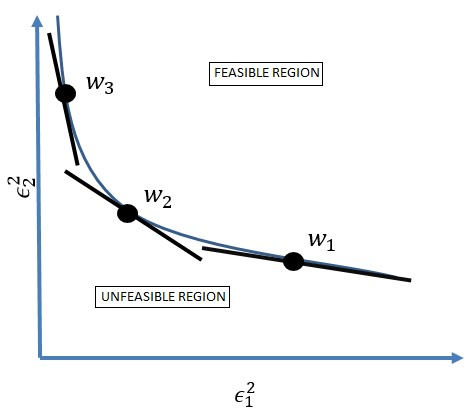
\includegraphics{chapter3/pareto_schematic}
  \caption{Schematic of a Pareto front for the differences, $\epsilon_1$ and $\epsilon_2$, between predicted and actual values for two arbitrary material properties.  The Pareto surface separates regions which are feasible and unfeasible.  Since points in the unfeasible region represent regions of unobtainable accuracy, the Pareto surface forms a boundary of the best possibilities with tradeoffs occurring on the convex hull. }
  \label{fig:pareto_convex}
\end{figure}

Figure \ref{fig:pareto_convex} provides a schematic in 2D, which allows us to illustrate this concept more concretely.  By the definition of Pareto optimality, the Pareto curve separates the feasible region from the infeasible region.  The points $w_1$, $w_2$. amd $w_3$ dominate some of the points on the interior of the Pareto curve, but they do not dominate each other.  The point $w_1$ has better performance with respect to $q_2$ at the expensive of $w_3$, while the fortunes are reserved for $w_3$.  The point $w_2$ is a compromise position between the two.  Without the expression of preferences, one is indifferent to the selection of any of these potentials, but it is rational to choose any of them since they are all Pareto efficient.  If an vector weights was chosen \emph{a priori}, then the potential developer is making a decision about the optimal parameterization without regard to tradeoffs in performance in the fitting set.

The shape of the Pareto front provides valuable insights into the performance of a potential formalism.  In this case, the Pareto front is monotonically decreasing and convex.    Suppose, we start with an initial set of weights $\bm{w}_1$, with the goal of reducing $\epsilon_1$.  A change in the weights to $\bm{w}_2$ places a larger preference on reducing $\epsilon_1$ at the expense of increasing $\epsilon_2$.  Due to the slope of the tangent line implied by the weights, a large reduction in $\epsilon_1$ is possible with only a small sacrifice in $\epsilon_2$.  However, continual improvements in reducing $\epsilon_1$ by changing the weights has a diminishing effect due to the convexity of the Pareto front.  A change in the weights from $\bm_{2}$ to $\bm{w}_3$ will still reduce $\epsilon_1$ at the expense of increasing $\epsilon_2$.  Compared to the previous change, a small reduction in $\epsilon_1$ comes with the tradeoff of a large increase in $\epsilon_2$.

\section{Multiobjective Optimization Methods}
A multi-objective optimization approach should achieve the following conflicting goals as described by Zitzler \emph{et al.} \cite{zitzler2000_moo_evolve}: (1) the best known Pareto front should be as close as possible to the true Pareto front.  Ideally, the best-known Pareto set should be a subset of the Pareto set, (2) solutions in the best known Pareto set should be uniformly distributed and diverse over the Pareto front in order to provide the decision-maker a true picture of trade-offs, and (3) the best-known Pareto front should capture the whole spectrum of the Pareto front at the extreme ends of the spectrum.  While the first two goals are important for multi-objective optimization, the last goal is erroneous.  In potential development, compromise solutions are desireable; a potential with high fidelity with respect to one material property at the expense of a loss of fidelity with respect to all other predictions is pathological.

\section{Solution Methods}
Weights that produce a certain Pareto optimal solution are not necessarily unique, and different weights may produce similar solutions.  On the other hand, a small change in weights may cause big differences in the objective function.  It is not easy for the potential developer to control the solution process because weights behave in an indirect way.  The solution process then becomes interactive, where one tries to guess the weights that would produce a satisfactory solution.  When the tools for potential development to not adequate to support the potential developer in such an \emph{ad hoc} approach, the process leads to frustration and complications in potential development.  In this case, it is advisable to develop a real interactive method where the solution process can be better controlled so that the potential developer can provide more intuitive preference information.

By calculating the Pareto set before analysis and selection, the whole problem of expressing preferences disappears and the traditional analysis approach can proceed in an interactive way.  In addition, provides a wealth of information into all the different rational parameterization, enabling applications such as parametric uncertainty as an input to feed foward to uncertainty quantification methods, shortcomings of potential formalisms, and correlations of errors between computationally inexpensive testing set QOIs to more expensive $T>0$ simulations, which are used to calculate key material properties in engineering applications and larger scale simulations.

\subsection{Pareto Optimization from Cost Function Optimization}

In potential development, the preferences of potential developer influences are particular parameterization, which has the result that the development of empirical potentials is somewhat of a black art.  Here, we demonstrate that the choice of using local optimization tools, as sparsely documented methods for overcoming the weaknesses of local optimization requires considerable skill and experience on the potential developer, as it is difficult to obtain the Pareto surface using traditional techniques.

Let us consider the unlikely case that our potential optimization problem, $C(\bm{\theta},\bm{w})$ is a convex function with respect to $\theta$ and $\nabla C$ being Lipschitz.  Then for an initial condition $\bm{\theta}_0$, we can numerically construct a sequence, ${\bm{\theta}_t}$,
\begin{equation}
	C(\bm{\theta}_{t+1}) < C(\bm{\theta}_{t}), \qquad t = 0,1...
\end{equation}
In each direction, we search in the descent direction informed by the gradient, $\nabla C(\bm{\theta}_t)$ by step size $\eta_t$ to determine $\bm{d}$, the distance to move.  In the gradient descent algorithm, the descent direction is $\bm{d}_t = - \nabla C(\bm{\theta}_t)$.  This process continues until convergence conditons are met to achieve the numerical approximation at $C(\bm{\theta}^*)$.  Any unique vector of weights $\bm{w}$ will result in the optimal parameterization with respect to the selection of weights.  Since $C(\bm{\theta}|\bm{w})$ evaluated at $\bm{\theta}^*$ is a constant, the vector of weights will also define the hyperplane tangent to the pareto surface,
\begin{equation}
	\sum_{i=1}^{N_Q} w_i L_i = C(\bm{\theta}^*)
\end{equation}

In the development of interatomic potentials, the DM is asked to specify weights in which case the method is used as an \emph{a priori} method.
To estimate the Pareto surface, it is sufficient to select a set of weightings.  Since our function is convex and Lipschitz, each unique selection of $\bm{w}$ will give a different point on the Pareto surface as the schematic in figure \ref{fig:pareto_convex}.

The weighting method can be used as an \emph{a posteriori} method where different weight can be used to generate different Pareto optimal solutions, and then themost satisfactory solution selected afterwards.  Systemic methods of perturbing the weights to obatain different Pareto optimal solutions are suggested (Chankong and Haimes 1983), but Das and Dennis 1997 illustrates that an evenly distributed set of weights does not necessarily produce an evenly distributed representation of the Pareto optimal set, even when the problem is convex.
%https://books.google.com/books?id=NHZqCQAAQBAJ&pg=PA1&source=gbs_toc_r&cad=4#v=onepage&q&f=false

The use of local optimization techniques in potential development are clear: local optimization methods are fast, can handle large scale problems, and are largely applicable to a large range of potentials, since they only require differentiability of the objective function and the constraint function\ref{boyd_convex_optimization}.  When Karush-Kuhn-Tucker conditions\cite{karush1939_kkt,kuhn1951_kkt} are met for the constrained optimization parameter optimation problem, solutions remain fairly computationally tractable because of the maturity of the technology and methods associated with gradient based methods and linear algebra techniques.

Algorithms for multiobjective optimization should produce Pareto optimal solutions, and that any Pareto optimal solution can be found.  In this respect, the weighting method has a serious shortcoming.  Any Pareto optimal solution can be found by altering weights only if the problem is convex.  Some Pareto optimal solutions of nonconvex problems cannot be found regardless of how the weights are selected.  In potential parameterization, the compromise is to give up seeking the optimal $\bm{\theta}$, which minimizes the objective over all feasible points.  To solve the problem as a constrained minimization problem with subject to the usual inequality and equality constraints, $g_i(\bm{\theta})$ and $h_j(\bm{\theta})$.  The problems of the weighting schemes have ben explored by the classical potential development community.\cite{martinez2013_fitting}  The method may jump from one vertex to anohter vertex leaving intermediate solutions undetected with relatively small changes in the weighting schemes.\cite{martinez2013_fitting}

Instead, the choice the process is to seek a point that is only locally optimal, which means that it minimizes the feasible points which are near it.  The disadvantages of local optimization methods go beyond not finding the true, globally optimum solution.  The initial guess, $\bm{\theta}_0$ is critical, and can greatly affect the objective value of the local solution.  Little information is provided on how far from the globally optimal solution the local solution is.  In addition, local optimization methods are sensitive to the choice of algorithm, algorithm parameter values, which maybe need to be adjusted based upon the $C$ to $\bm{theta}$ response surface.

One way to overcome the problem with poor initial conditions, is to optimize the cost function from multiple initial conditions.  Given the upper and lower bound of $\bm{\Theta}$ for each parameter $\bm{\theta}$, one can construct an a a grid of initial conditions from which to start the local optimization routine.  As we will demonstrate later, this technique is computationally expensive as the gradient descent paths from each initial condition to achieve optimal solution, $\bm{\theta}^*(\bm{\theta}_0,\bm{w})$, which grows with the density of the grid, the dimensionality of the $q$-space, and the dimensionality of $\theta$-space.

As a result, potential developers have begun to experiment with global optimization techniques, such as genetic algorithms and simulated annealing\cite{martinez2013_fitting,martinez2016_posmat}, to obtain a true global solution of the optimization problem.  However, the compromise in these cases is efficiency.  As the potential formalism increases, the computational complexity of global optimization techniques also increases exponentially.

\section{Pareto Optimization from Monte Carlo techniques}

Genetic algorithms are a popular meta-heuristic that is particularly well-suited for this class of problems.  Traditional GA are customized to accomodate multi-objective problems by using specialized fitness functions and introducing methods to promote solution diversity.  The method which will be proposed in chapter 5 is not a genetic algorithm, but is designed as an evolutionary algorithm which reduces the epistemic uncertainty of parameterization, but evolving the distribution into a distribution  which describes the parameters which produces Pareto optimal results.

The previous section described how the Pareto surface could be estimated for a convex cost function, by selecting an initial condition and solving for the optimal parameterization given set of weights, then repeating the process by varying the weighting scheme.  However, when the cost function is not convex, the process becomes a local solution process and more computationally expensive techniques are necessary.  This can involve assessing multiple starting parameterizations and applying global optimization techniques.  More problematically, much of the information calculated from many evaluations of the cost function other than the final solution (given an initial condition and a weighting vector) is lost.  Even if the information was retained, it is unclear how to integrate that information to more efficiently calculate a Pareto surface.

In a deterministic approach we would want to identify an algorithm such that we start with feasible set of parameterizations and constrains the sets of parameterizations until it produces a set of parameterizations which produces a set of optimal parameters $\bm{\Theta}^*$, which produces Pareto-optimal results $\epsilon$-space.  Here we propose a technique that takes advantage of Monte Carlo sampling.  While Monte Carlo solutions converge slowly, the error of estimamtion decreases as $1/\sqrt{N}$, unlike deterministic search methods that depend expend exponentially on the dimension\cite{caflisch1998_mc}.

The main idea behind this method is that results are based on repeated sampling.  Here we assume that $\bm{\Theta}$ is a random variable, with a probability distribution function which encompasses the information we know about the parameter space.  When we have much information about the parameters, we can use a uniform distribution defined by upper bound and lower bound for each parameter.  Since $\bm{\theta}$ is now a realization of the random variable $\bm{\Theta}$, for each $\bm{\theta}_i$ we can produce $\hat{\bm{q}}_i(\bm{\theta})$ by running these simulations against our simulation machinery.  Moreover, this method is trivially parallelizable.

To determine the estimate $\bm{\Theta}^*$ is determined the following algorithm.  Given the set of QOI evaluations, $\hat{\bm{Q}}=\{\hat{\bm{q}}()\bm{\theta}_1),...,\hat{\bm{q}}_i{\theta}\}$ calculate the Pareto optimal set using the definition of the Pareto optimality, $\hat{\bm{Q}}^* \subseteq \hat{\bm{Q}}$.   The parameters which produce the elements in $\hat{\bm{Q}}^*$, are the set of parameters which produce the Pareto optimal parameters.

The convergence of this algorithm can be drastically improved by updating the probability distribution based upon the results of previous simulations.  In chapter 5, we discuss this process in more detail.

\subsection{Computational and Performance Comparison}
 The performance of these algorithms were tested against the well known problems of Schaffer\cite{schaffer1984_pareto} and Kurasawe\cite{kursawe1001_pareto} to demonstrate the relative performance computational cost of these approaches.  Both of these problem only have two objective functions, which makes visualization of the concepts more concrete.

 awe can produce as many samples to evaluate for performance against the fitting database to produce $\bm{q}.$  When a large enough amount of samples are evaluated,
 It is a generic solution and the iterative approach of generating new populations is akin to previous solutions.
 increases with the increase in the number of objectives.

 The ultimate goal of a multi-objective optimization algorithm is to identify solution in the Pareto optimal set.  However, identifiying the entire Pareto optimal set, for multi-objective problems, is impossible to its size.  Proof of solution optimality is computationally infeasible.  Therefore, a practical approach is achieve successively better approximations of the Pareto surface that represent the Pareto set as well as possible.

 The first of the test optimization function of a smooth convex multi-objective optimization problem described by Schaffer\cite{schaffer1984_pareto}.  Here the multi-objective function $F:\mathbb{R} \rightarrow \mathbb{R}^2$.
 \begin{equation}
 \begin{aligned}
   &\min_{x}
       \begin{aligned}
            &f_1(x) = x^2 \\
            &f_2(x) = (x-2)^2 \\
       \end{aligned}
 \end{aligned}
 \end{equation}

The second test optimization problem of Kurasawe.
begin{equation}
\begin{aligned}
  &\min_{\bm{x}}
    \begin{aligned}[t]
      &f_(\bm{x}) = \sum_{i=1}^2
          \left[
            -10 \exp\left(-0.2 \sqrt{x_i^2} + x_{i+1^2}\right)
          \right] \\
      &f_x(\bm{x}) = \sum_{i=1}^3 \left[ \vert|x_{i} \vert|^{0.8} + 5\sin(x_i^3)\right] \\
    \end{aligned}
  &\text{subject to} \\
    \begin{aligned}[t]
      &-5 \leq x_i \leq -5 \\
      & 1 \leq i \leq 3 \\
    \end{aligned}
  \end{aligned}
\end{equation}


\begin{table}
\caption{Computational comparison between gradient methods and simulation methods against the Kurasawe MOO problem.-+++++}
\label{table:kurasawe}
\begin{tabularx}{6.5 in}{c c c c}
	\hline
  & & CG method & MC method & KDE method \\
	\hline
	Function Evaluations &1053132 &100000 &100000
	Pareto points & 22 & 311
	\hline
\end{tabularx}
\end{table}
